\documentclass{article}
\usepackage[margin=1.5cm,bottom=2cm]{geometry}
\usepackage{fancyhdr}
\usepackage{graphicx}
\pagestyle{fancy}

\begin{document}
\fancyhead[L]{ 
\includegraphics[width=2cm]{au_logo.png} }
\fancyhead[R]{PHYS 2250: General Physics II}
\fancyfoot[C]{\thepage}
\vspace*{0cm}
\begin{center}
	{\LARGE \textbf{Homework 0}}\\
	\vspace{0.25cm}
	{\Large Due: Friday, September 4}
\end{center}

\begin{enumerate}
	\item Calculate the magnitude of the vector $\vec{A}=<3,5,1>$
	\item The position of an electron is given by $\vec{r}_e=4\hat{x} - 2\hat{z}$ and the position of a proton is given by $\vec{r}_p=2\hat{y} + 3\hat{z}$. Find the vector which describes the position of the electron \textit{relative to} the position of the proton.
	\item Let $\vec{A}=<9,5,8>$ and $\vec{B}=<-3,-5,4>$. What is $\vec{A}\cdot\vec{B}$? What is the angle between these two vectors?
	\item What is the unit vector describing the direction of the vector $<-3,7,1>$? What is the angle of this vector with respect to the positive x-axis?
	\item Let vector $\vec{B}=3\hat{x}-9\hat{y}+7\hat{z}$ and $\vec{v}=8\hat{x}+4\hat{y}+6\hat{z}$. Find the vector $\vec{F}=\vec{B}\times\vec{v}$
	\item Are the vectors $\vec{A}=<4,5,-7>$ and $\vec{B}=<6,-2,2>$ orthogonal?
	\item A metal bar of length $L$ has its mass distributed evenly with a constant mass per unit length $\lambda=\lambda_0$. What is the mass of the bar?
	\item A second metal bar of length $L$ has its mass distributed as a function of distance from the edge of the bar: $\lambda(x)=\lambda_0 \left(\frac{x}{L}\right)^3$. What is the mass of this bar?
	\item\label{problem_circle} A metal wire of length $L$ is bent into a circle such that the linear mass density (mass per unit length) is given as a function of the angle $\phi$ (see Figure \ref{circle_bar}) as $\lambda(\phi)=\lambda_0\phi$. What is the mass of the bar?
	
	\begin{figure}[ht!]
		\centering
		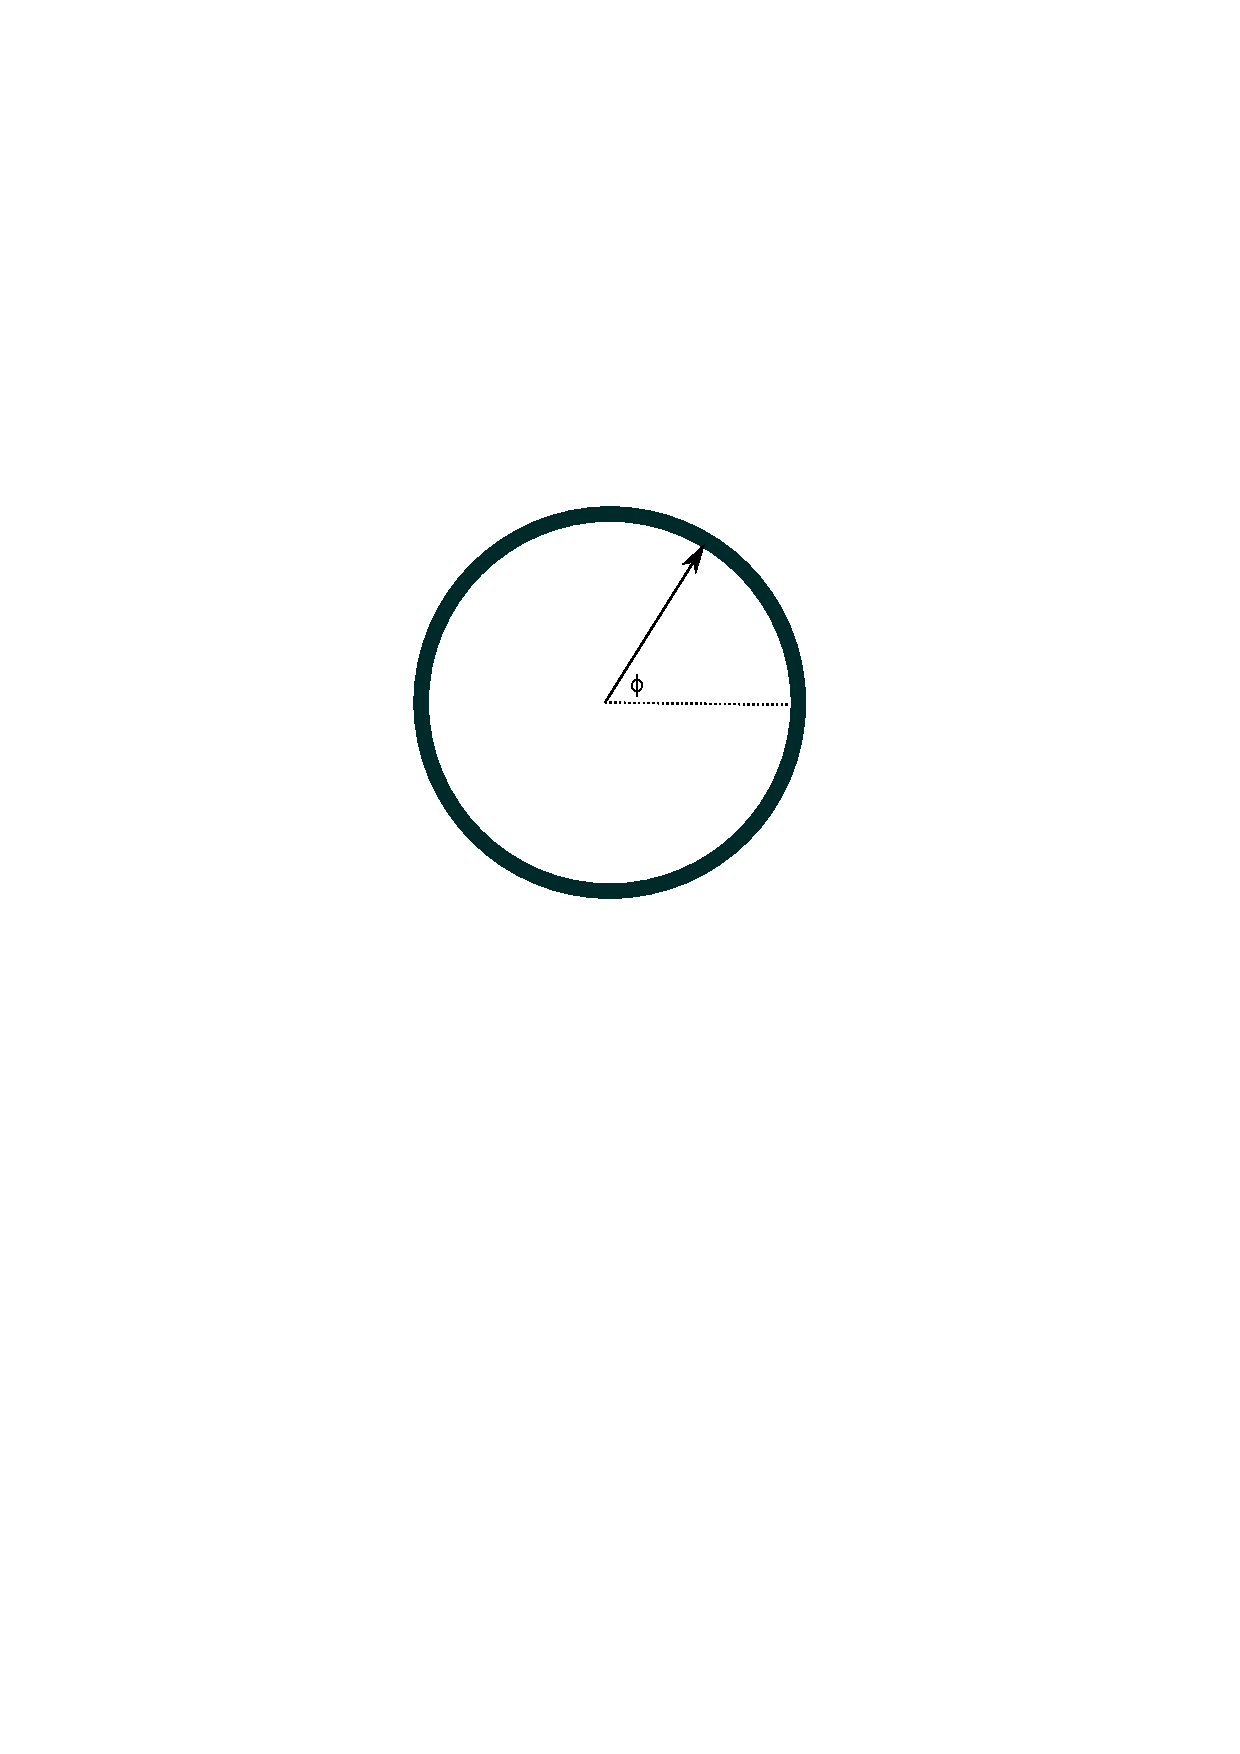
\includegraphics[width=0.3\textwidth]{circle_bar}
		\caption{Diagram for problem \ref{problem_circle}.}
		\label{circle_bar}
	\end{figure}

	\item A solid disk of radius $R$ has mass per unit area distributed as $\sigma(r)=\sigma_0 \left(\frac{r}{R}\right)^2$. What is the mass of the disk?
	\item A solid sphere of radius $R$ has mass per unit volume distributed as $\rho(r)=\rho_0 \left(\frac{r}{R}\right)$. What is the mass of the sphere?
\end{enumerate}

\end{document}